%Note di Ingegneria del Software
%Sommario: UML, Diagrammi dei casi d'uso, estensioni, inclusioni, generalizzazioni

\cornell{UML}{Unified Modeling Language\\
Insieme di notazioni grafiche (si usano disegni invece di sole parole in linguaggio naturale), pensato su un paradigma ad oggetti (object oriented).\\
Come Editor di riferimento in questo corso useremo Papyrus (http://www.eclipse.org/papyrus)}
\cornell{Uso di UML}{\begin{itemize}
\item Come abbozzo (sketch): il modo più usato
\item Come progetto: Inserendolo dentro la documentazione ed usandolo come base per il progetto
\item Come linguaggio di programmazione: Così da poter generare codice automaticamente, partendo da UML.\\
Così da avere un software provato (anche matematicamente)
\end{itemize}}
\cornell{Diagrammi dei casi d'uso}{Sono usati nella fase di analisi.\\
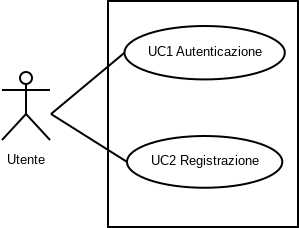
\includegraphics[scale=0.5]{images/10.png}\\
Legenda:\\
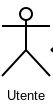
\includegraphics[scale=1]{images/11.png} \textbf{Attore o Ruolo:} Chiunque agisca \underline{dall'esterno} sul nostro software\\
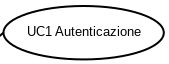
\includegraphics[scale=1]{images/12.png} \textbf{Funzione/Caso D'uso} Solitamente accompagnato da un identificatore (In questo caso UC1) a cui si fa riferimento nella descrizione.\\
Per relazionare attori e casi d'uso si usa una linea \textbf{continua non direzionata}}
\cornell{Dettaglio dei casi d'uso}{
Posso poi entrare in maggior dettaglio, nei vari casi d'uso, come per la registrazione:\\
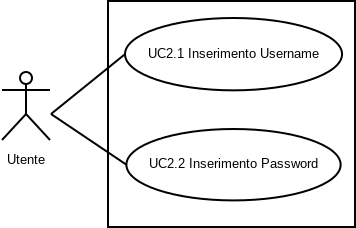
\includegraphics[scale=0.5]{images/13.png}\\
Notare come gli identificatori cambiano, in maniera gerarchica (UC2.1, che è evidentemente parte di UC2).\\
Quando sono arrivato al massimo livello di dettaglio, è semplice arrivare ai requisiti.
}
\cornell{Estensione}{Usata solitamente per modellare casistiche di errore.\\
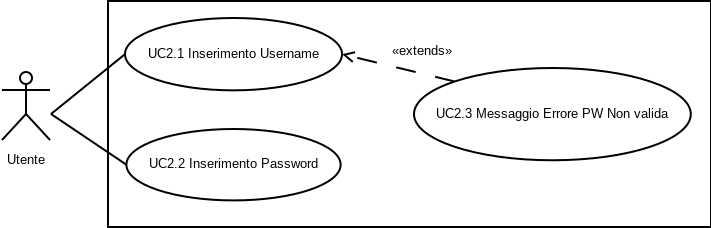
\includegraphics[scale=0.4]{images/14.png}\\
Si relaziona con una \textbf{linea tratteggiata direzionata} verso la classe estesa.\\
La parola chiave $\langle \langle$ extends $\rangle \rangle$ è detta \textbf{direttiva UML}\\
L'esecuzione del caso d'uso da cui si estende \textbf{viene interrotta} e non arriva al termine.\\
Si aggiunge inoltre la condizione per arrivare all'estensione all'interno del caso d'uso da estendere oppure in una primitiva "commento"\\
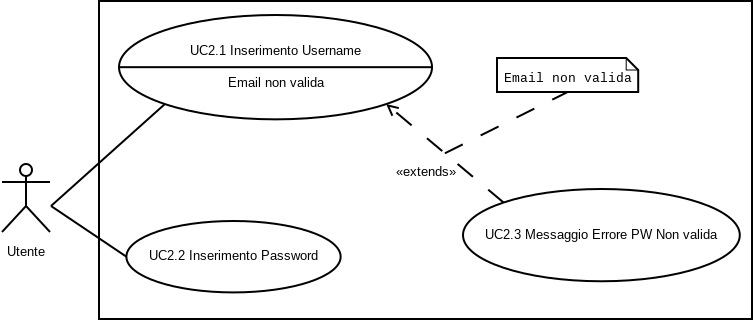
\includegraphics[scale=0.4]{images/15.png}}
\cornell{Scenario}{Sequenza di passi che descrivono interazioni.}
\cornell{Screnario Principale}{Sequenza normale di operazioni che si eseguono "se tutto va bene"}
\cornell{Scenari Alternativi}{Rappresentano scenari possibili diversi dallo scenario principale (ad esempio il messaggio di errore della mail non valida)}
\cornell{Casi D'uso}{Specifiche testuali dei casi d'uso, molto più informative del diagramma.\\
Specificano anche gli attori secondari, pre- e post-condizioni, descrizione dettagliata dello scenario principale e delle estensioni.\\
Esempio:\\
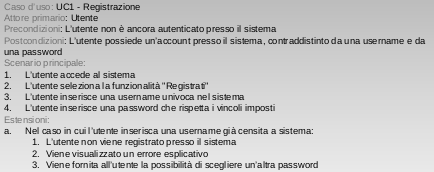
\includegraphics[scale=0.7]{images/16.png}}
\cornell{Attori}{Persona o sistema esterno che interagisce con il nostro sistema.\\
In un sistema solitamente vi sono più attori, a seconda delle precondizioni con cui ci troviamo a lavorare.\\
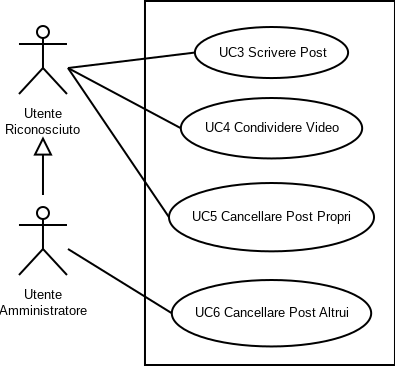
\includegraphics[scale=0.5]{images/17.png}}
\cornell{Subclassing (o Generalizzazione)}{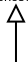
\includegraphics[scale=1]{images/18.png} con una freccia continua che termina in un triangolo vuoto, si definisce una generalizzazione tra attori (non è il subclassing della programmazione), nel caso visto prima possiamo vedere che l'utente amministratore ha le funzionalità di utente riconosciuto, più qualche altra.\\
È possibile avere anche generalizzazioni tra casi d'uso.\\
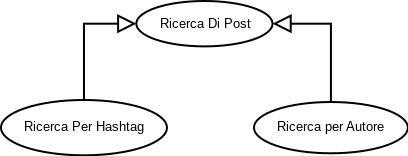
\includegraphics[scale=0.5]{images/19.png}}
\cornell{Inclusione}{Ogniqualvolta un attore accede ad un caso d'uso, dopo che questo si conclude, viene eseguito \textbf{incondizionatamente} un altro caso d'uso.\\
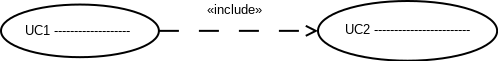
\includegraphics[scale=0.5]{images/20.png}\\
La direzione della freccia tratteggiata va verso il caso d'uso eseguito.\\
Viene usato per seguire il principio DRY (Don't repeat yourself).}
